\documentclass[iop, apj]{emulateapj}

\usepackage{fancyhdr}
\usepackage{extramarks}
\usepackage{amsmath}
\usepackage{amsthm}
\usepackage{amsfonts}
\usepackage{mathtools}
\usepackage[makeroom]{cancel}
\usepackage{fullpage}
\usepackage{graphicx}
\usepackage{epstopdf}
\usepackage{prettyref}
\usepackage{enumerate}
\usepackage[bookmarks]{hyperref}
\usepackage{grffile}
\usepackage[super]{nth}

\slugcomment{AMS250 Final Project}

\shorttitle{Game of Life}
\shortauthors{Eric Gentry}

\begin{document}

\title{Parallelizing Conway's Game of Life}

\author{Eric Gentry}
\email{egentry@ucsc.edu}

\section{Introduction}

For this final project, we were given the task of programming a parallel version of Conway's \emph{Game of Life}.  The rules to the Game of Life are simple and relatively well known and will not be discussed here (for details, see \href{https://en.wikipedia.org/wiki/Conway\%27s_Game_of_Life}{wikipedia}). Our primary challenge was to write and parallelize a Game of Life simulator.  Ideally, it should scale well to an arbitrary number of cores.

The code written and used for this project is available at \url{https://github.com/egentry/Game_of_Life}.  Section \ref{sec:PCAM} will go into details about the algorithmic choices behind this project. Section \ref{sec:model} will evaluate the algorithmic design choices in terms of theoretical models and empirical performance data.

\section{PCAM}
\label{sec:PCAM}

This section seeks to explain the design choices under the ``Partitioning -- Communication -- Agglomeration -- Mapping'' framework (\emph{PCAM}).

\subsection{Partitioning}

At the atomic level, every location on a 2D grid needs to be evolved to a new state, using information from the old states of the surrounding 8 neighboring cells.  Within a timestep, any cell can be updated in any order.  This update step, which is done for each cell location, is the finest level of partitioning appropriate for this problem.

\subsection{Communication}

Each of our tasks requires knowledge of the old states of the 8 surrounding neighbors; local channels to each of those neighbors are required for this information.  Within a timestep, this communication can take place in any order. Extra care needs to be taken in adhering to periodic boundary conditions --- no boundary conditions need to be enforce, so long as channels are created between appropriate tasks on the boundaries of the overall computational domain.  The only global communication required is for Input/Output tasks.

\subsection{Agglomeration}

A typical node can handle updating far more than a single grid point.  By agglomerating we can increase the amount of cells we can evolve for a fixed number of processors, and by agglomerating well we can minimize the communication required per computation.

The communication in this problem is entirely local, which means only the boundaries of a computational domain need to be communicated.  In order to minimize the communication (related to the size of the boundary) per computation (related to the area of the domain), we effectively have a ``surface area-to-volume'' problem.  Since this task-channel structure is analogous to fixed grid hydrodynamical solvers, we know the best way to minimize ``surface area-to-volume'' is to decompose in the dimensionality of the problem.  We have a 2-dimensional problem, so we want to decompose and agglomerate tasks in 2-dimensions. For ideal performance, grid points should be agglomerated into rectangles within the computational domain.

Since this problem is a fixed grid, with fixed computation per grid point, we also expect the loads on each processor to be relatively static (with the exception being I/O related processors). Given this static load, we do not expect load re-balancing to necessary.

\subsection{Mapping}

In short, much of the mapping will be left to MPI and the batch system on Grape, the Applied Math and Statistics compute cluster at UCSC.  Using the batch system we will requires a number of nodes, and will use all the cores on each node. This will minimize the inter-node communication, which will be slower than intra-node communication. Alternatively, we could have used a hybrid model, using \texttt{MPI} between nodes,
and \texttt{OpenMP} within nodes, but for simplicity we have kept a single programming model.

Once allocated nodes and cores, the only further mapping might happen when we create a Cartesian virtual communication topology within \texttt{MPI}.  We will allow \texttt{MPI\_Cart\_create} to reorder processor ranks with the knowledge of how we plan to communicate, but this only allows for the opportunity of re-mapping cores.  Re-mapping is not guaranteed.

\section{Performance Model}
\label{sec:model}

In this section, we will construct a \emph{wall-clock} runtime model.  We'll then make and test predictions regarding the weak scaling of our model.

\subsection{Theory}

As discussed in in Section \ref{sec:PCAM}, $N$ tasks are agglomerated in rectangular sub-domains of size $N_x$ by $N_y$, with $n_{gc}$ guard cells of padding in each dimension. For simplicity, we'll enforce $N_x = N_y = \sqrt{N}$.  The number of ``true'' cells in each sub-domain is then:
\begin{equation}
N_\mathrm{true} = (N_x - n_{gc}) (N_y - n_{gc} ) = ( \sqrt{N} - n_{gc})^2
\end{equation}
but in order to make full use of the guard cells (when $n_{gc} > 1$), we'll need to do a variable number of calculations each timestep.  If all of our guard cells are accurate, then we can do $( \sqrt{N} - 1)^2$ updates; the next time step we can do $( \sqrt{N} -2)^2$ time steps, until we are left with just the ``true cells'' where we do $( \sqrt{N} - n_{gc})^2$ updates.  At that point we will need to communicate with nearby cells to refresh our guard cell information.  But before thinking about communication, let's find the average time spent updating cells.  The average number of cells updated per cycle is:
\begin{align}
	\langle N \rangle_\mathrm{update} &= \frac{1}{n_{gc}} \sum\limits_{i=1}^{n_{gc}} (N_x -i)(N_y - i)
	\\
	\langle N \rangle_\mathrm{update} &= \frac{1 - 6 \sqrt{N} + 6 N + 3 n_{gc} - 6 \sqrt{N} n_{gc} + 2 n_{gc}^2}{6}
\end{align}
This will result in an average computational time:
\begin{equation}
	T_\mathrm{comp} = t_\mathrm{update} \langle N \rangle_\mathrm{update}
\end{equation}
(We will use the convention $T_i$ referring to the \emph{total} wall-clock time spent doing type of action $i$ within a single cycle. Similarly, $t_i$ will be the time per task within the overall action.)

Every $n_{gc}$ time steps, we will need to communicate between adjacent sub-domains to update guard cells.
For communication we expect both start-up costs $t_\mathrm{start}$ and length-dependent costs $t_\mathrm{size}$.  Each sub-domain will need to communicate $n_{gc}$ rows or columns in 4 directions. This will incur an average $4 t_\mathrm{start}$ per time step, as well as the length-dependent costs $2 (N_x + N_y) t_\mathrm{size}$, where $t_\mathrm{size}$ is the cost per variable communicated, and $2 (N_x + N_y)$ is the perimeter (total size of the messages communicated). (Time per communication will be expected to be $n_{gc}$ times longer, but will only need to run once every $n_{gc}$ time steps.) For simplicity, we will assume the constants $t_\mathrm{start}$ and $t_\mathrm{size}$ are the same between all processors, even though this is not true for the physical network topology.

This brings our average total time cost to:
\begin{align}
	T &=  T_\mathrm{comm} + T_\mathrm{comp}
	\\
	&=  4 t_\mathrm{start} + 4\sqrt{N} t_\mathrm{size} + t_\mathrm{update} \langle N \rangle_\mathrm{update}
	\\
	&= 4 t_\mathrm{start} + 4\sqrt{N} t_\mathrm{size} 
	\\ \nonumber &+ t_\mathrm{update} \frac{1 - 6 \sqrt{N} + 6 N + 3 n_{gc} - 6 \sqrt{N} n_{gc} + 2 n_{gc}^2}{6}
\end{align}

This is ugly, but it's worth pointing out a few key features. At no point does our time model depend on the number of processors, $P$.  That is because we have formulated our model in a way that makes a weak scaling test natural. (It also simplifies the design, as agglomeration need not depend on the number of processors.)
Secondly, for fixed $N$, we expect $T$ to drop with increasing $n_{gc}$, and we expect it to keep dropping for all $n_{gc} < \sqrt{N}$. This indicates that our model is insufficient for yielding useful information about how to optimize the choice of $n_{gc}$.  If we set $n_{gc} = \sqrt{N}$ we get the minimal $T$, but we will just be running identical copies of the same domain on every processor --- we will have the serial case.  For a more meaningful result, we should consider the total \emph{wall-clock} time per ``true'' cell on each processor, which we will term $\tau$

\begin{align}
	\tau &\equiv \frac{T}{N_\mathrm{true}}
	\\
	&= \frac{1}{(\sqrt{N} - n_{gc})^2} \left( 4 t_\mathrm{start} + 4\sqrt{N} t_\mathrm{size} \right. \label{eq:performancemodel}
	\\ \nonumber & \left.+ t_\mathrm{update} \frac{1 - 6 \sqrt{N} + 6 N + 3 n_{gc} - 6 \sqrt{N} n_{gc} + 2 n_{gc}^2}{6} \right)
\end{align}

Now we have our theoretical model, and if given constants for $t_\mathrm{start}, t_\mathrm{size}, t_\mathrm{update}$ we can either run a weak scaling test, and if that is successful, use our model to choose an optimal number for $n_{gc}$.

\subsection{Verification}

Using my code, I ran tests on Grape to determine the constants:
\begin{align}
	t_\mathrm{start} &= 3.73 \cdot 10^{-5} \text{ s}
	\\
	t_\mathrm{size} &= 3.56 \cdot 10^{-9} \text{ s / \texttt{short}}
	\\
	t_\mathrm{update} &=6.60 \cdot 10^{-9} \text{ s / timestep / true grid point}
\end{align}
(These constants were all determined using multiple processors on one node. Only using one node will introduce errors which we will discuss later.)

\subsubsection{Weak Scaling}
On Grape, I ran weak scaling test ranging from 1 processor to 64 processors (8 nodes, of 8 processors per node), running for 100 timesteps, with a $1024 \times 1024$ grid on each process with 1 guard cell of padding on each edge (i.e. $(1024 - 2)^2$ true grid points). The results can be seen in Figure \ref{fig:weakscaling}. For a small number of processors ($\leq 8$), the results are relatively close to the prediction made by our performance model.  Unfortunately, once we use greater than 8 processors (requiring multiple nodes) we find that performance begins to suffer significantly.  This is likely due to the additional cost of communicating between physical nodes, which is more costly than communicating between processors on the same node.

\begin{figure}[tbp]
\centering
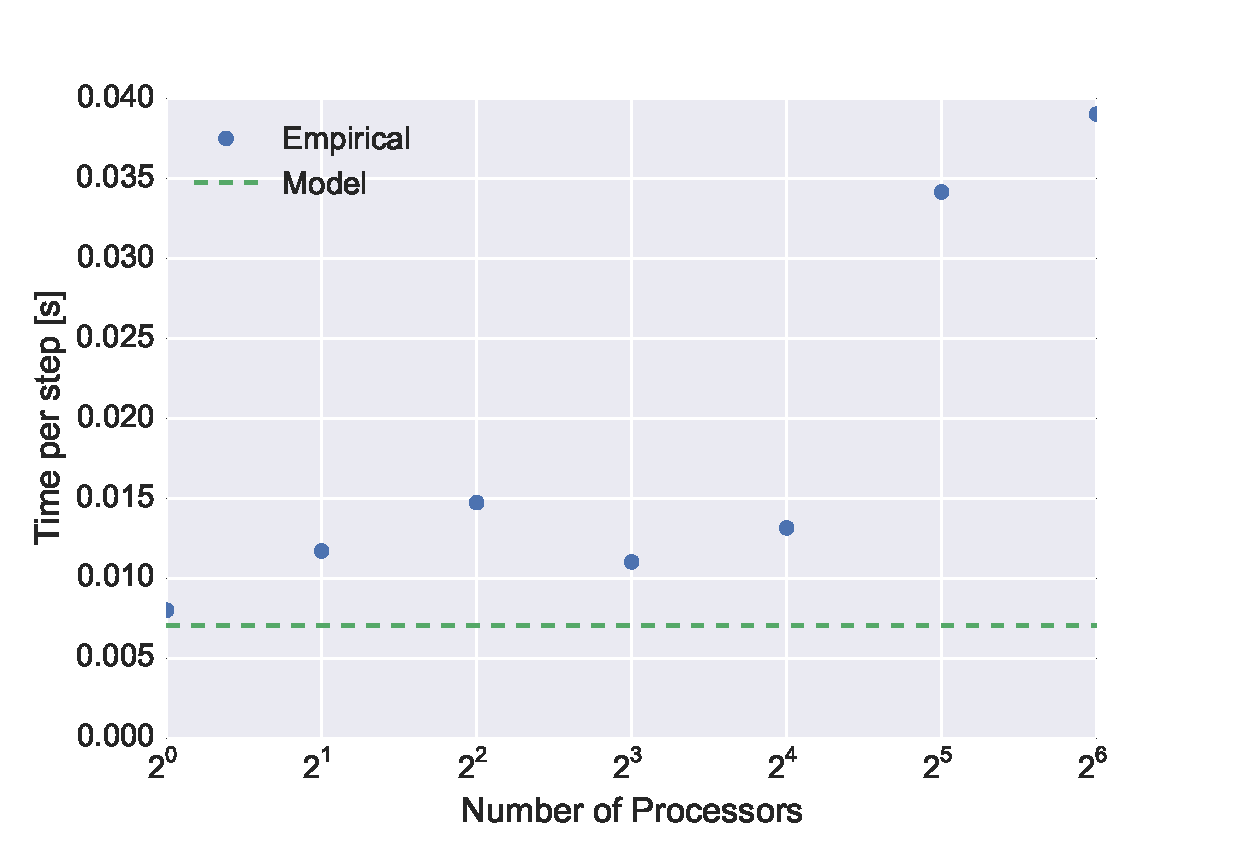
\includegraphics[width=\linewidth]{plots/weak_scaling.eps} 
\caption{ Weak scaling tests, ranging from 1 processor to 64 processors.  Equation \ref{eq:performancemodel} was used as our performance model, with empirically determined constants. }
\label{fig:weakscaling}
\end{figure}

\subsubsection{Guard Cell Scaling}
As noted above, I was interested in how the number of guard cells affected performance.  Using 64 processors (8 nodes of 8 processors each), I ran tests with 1 through 64 guard cells, running 100 evolution steps. Results can be seen in Figure \ref{fig:guardcell}.  The data are significantly worse than the performance model we constructed in Equation \ref{eq:performancemodel}.  This worse performance appears to be entirely due to the effect of using multiple node, while benchmarking on only one node (compare the benchmarked time for 64 processors in Figure \ref{fig:weakscaling} to the times shown in Figure \ref{fig:guardcell}).

\begin{figure}[tbp]
\centering
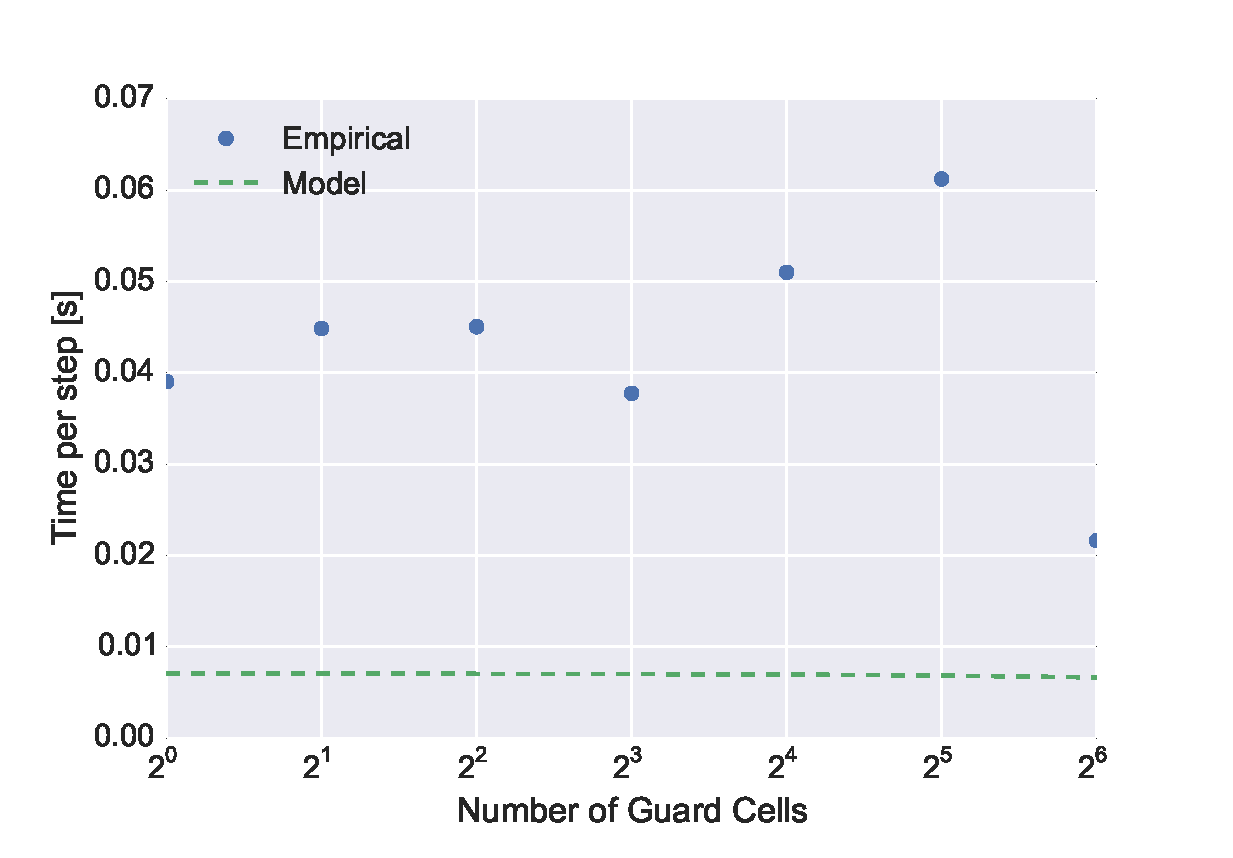
\includegraphics[width=\linewidth]{plots/guard_cell_scaling.eps} 
\caption{ Weak scaling tests, ranging from 1 processor to 64 processors. }
\label{fig:guardcell}
\end{figure}

It should be noted that our performance models, once the appropriate constants were determined, suggested very little change in runtime as a function of number of guard cells.  This is unsurprisingly, because our communication times are still dominated by the startup, even for a $1024^2$ grid.  Furthermore, I did not optimally package the sending of guard rows / columns into a single communication. Instead, I made a new send/receive call for each guard row / column.  In the future, proper buffering of multiple guard rows / columns would be more appropriate.

\section{Discussion}
I was successful in constructing a parallel solver for Conway's Game of Life, with a 2D domain decomposition.  For a small number of processors, the runtime is dominated by processing time and is accurately predicted by our performance model.  As we use use more nodes, we find that communication costs begin to rise, which was not predicted by my model.  A better performance model might seperately include \emph{intra-node} communication costs and \emph{inter-node} communication costs.

The inter-node communication costs lead to an interest possibility with regards to our guard cell scaling.  Our performance model would predict that the number of guard cells shouldn't affect the runtime significantly, since the model predicted that computational costs would dominate the runtime.  But, since communication costs dominate the runtime for large numbers of processors, a greater number of guard cells might be a way to minimize these costs.  Unfortunately, my guard cells were not sufficiently well implemented to test this possibility; it remains just a hypothesis.


%%%%%% SAMPLE FIGURE SNIPPET
% \begin{figure}[htbp]
% \centering
% \includegraphics[width=.7\textwidth]{../plots/surface_of_section.eps} 
% \caption{ Surface of section, sliced when the orbit crosses from $y<0$ to $y>0$.  }
% \label{fig:surfaceofsection}
% \end{figure}

\end{document}